% arara: pdflatex: {synctex:on}
% arara: biber
	% arara: pdflatex: {synctex:on}
% arara: pdflatex: {synctex:on}

\documentclass[11pt,oneside,toc=bibliography,a4paper]{scrbook}

%MARGINS AND SPACING
\usepackage[left=40mm,top=25mm,bottom=30mm,right=17mm]{geometry}
\usepackage[doublespacing]{setspace}
\clubpenalty = 10000
\widowpenalty = 10000
%ACRONYMS
\usepackage[acronym,nonumberlist,sort=def]{glossaries}
%\loadglsentries{Setup/acronyms}
\makenoidxglossaries
%\setacronymstyle{long-short}
\setglossarystyle{tree}
\usepackage[none]{hyphenat}\sloppy
\usepackage{verbatim}
\usepackage{graphicx}
\usepackage{enumitem}
\setlist{noitemsep}
\usepackage{tabulary}

%FONTS

%\usepackage[T1]{fontenc}
%\usepackage[utf8]{inputenc}

%\usepackage[sc]{mathpazo}
%\usepackage{eulervm}
%\usepackage{helvet}
%\usepackage{ebgaramond}

\usepackage{fontspec}
%\setmainfont{Times}

%\setmainfont{Calibri}

%\setmainfont{Helvetica}
%\setsansfont{Helvetica}

\setmainfont{Athelas}
\setsansfont{Athelas}

%\setmainfont{Futura}
%\setsansfont{Futura}


%\renewcommand{\sfdefault}{ptm} %heading font
%\renewcommand{\rmdefault}{ptm} %body font

%	UWE Harvard BibLaTeX formatting
%
%	To use this formatting, store this file in your tex documents 
%	directory and include %	UWE Harvard BibLaTeX formatting
%
%	To use this formatting, store this file in your tex documents 
%	directory and include %	UWE Harvard BibLaTeX formatting
%
%	To use this formatting, store this file in your tex documents 
%	directory and include \input{uweharvard} in the preamble, and use \addbibresource{•} and \printbibliography in your document.
%
%   Make sure to run biber instead of bibtex.
%	In texmaker, go to Preferences -> Commands, change the Bib(la)tex field from "bibtex" % to "biber" %
%
%	Use the \citep{} and \citet{} cite commands
%	\citep{} does name first then date in brackets
%	\citet{} does name and date in brackets.
%	This is incomplete, but formats webpages, articles, 
%	books, theses, incollections and inproceedings correctly. 
%	Feel free to add more!
%
\usepackage[natbib = true,
			sorting=nyt,
			citestyle = authoryear,
			bibstyle = authoryear,
			maxcitenames = 3, 
			mincitenames = 1,
			maxbibnames = 99,
			uniquename = false,
			uniquelist = false,
			firstinits = true,
			backend = biber,
			date = long
			]
			{biblatex}

\defbibenvironment{bibliography}
{\list
	{}
	{\setlength{\leftmargin}{\bibhang}%
	\setlength{\itemindent}{-\leftmargin}%
	\setlength{\itemsep}{\bibitemsep}%
	\setlength{\parsep}{\bibparsep}}}
	{\endlist}
	{\item}
	
\newbibmacro*{begentry}{}
\newbibmacro*{finentry}{\adddot}

\DefineBibliographyStrings{english}{%
    andothers = {\em et\addabbrvspace al\adddot}
}

%\DeclareBibliographyDriver{}{%
%	\usebibmacro{begentry}
%	
%	\usebibmacro{finentry}
%}

\DeclareSourcemap{
	\maps[datatype=bibtex]{
		\map{
			\pertype{inbook}
			\step[fieldsource=bookyear,fieldtarget=note]		
		}	
	}
}

\DeclareFieldFormat{edition}%
                   {\ifinteger{#1}%
                    {\ifnumequal{#1}{1}
                    {}
                    {\mkbibordedition{#1}\addthinspace{}ed.}}%
                    {#1\isdot}}
                    
\DeclareNameAlias{sortname}{last-first}
\DeclareFieldFormat[book,article,inproceedings,thesis,incollection,webpage,inbook]{year}{\mkbibparens{#1}}
\DeclareFieldFormat[inbook]{note}{\mkbibparens{#1}}
\DeclareFieldFormat[thesis]{title}{\emph{#1}}
\DeclareFieldFormat[inproceedings,article,incollection]{title}{#1}
\DeclareFieldFormat[inproceedings, incollection]{booktitle}{\printtext{In:}\addspace\emph{#1}}
\DeclareFieldFormat[inbook]{title}{\emph{#1}}
\DeclareFieldFormat{chapter}{#1}
\DeclareFieldFormat[article]{journaltitle}{\emph{#1}}
\DeclareFieldFormat[webpage]{title}{\emph{#1}}
\DeclareFieldFormat[webpage]{url}{\printtext{Available From:}\addspace\url{#1}}
%\DeclareFieldFormat[webpage]{lastchecked}{\mkbibbrackets{Last Accessed: #1}}
\DeclareFieldFormat[webpage]{lastchecked}{\mkbibbrackets{#1}}
\DeclareFieldFormat[webpage]{note}{\mkbibbrackets{#1}}
\DeclareFieldFormat[article]{number}{\mkbibparens{#1}}

\DeclareFieldFormat{language}{\printtext{Translated from }\addspace{#1}}
\DeclareFieldFormat{translator}{\printtext{by }\addspace{#1}}


\DefineBibliographyStrings{english}{%
	page={\printtext{p.}},
	pages={\printtext{pp.}},
}


\DeclareBibliographyDriver{webpage}{%
	\usebibmacro{begentry}
	\printnames{author}
	\newunit
	\printlist{organization}
	\setunit*{\addspace}\newblock
	\printfield{year}
	\setunit*{\addspace}
	\printfield{title}
	\newunit\newblock
	\printfield{url}
	\setunit*{\addspace}\newblock
	\printfield{note}
	\printfield{lastchecked}
%	\printfield{Date-Added}
	\usebibmacro{finentry}
}

\DeclareBibliographyDriver{inbook}{%
	\usebibmacro{begentry}
	\printnames{author}
	\newunit
	\printfield{year}
	\setunit*{\addspace}\newblock
	\printfield{chapter}
	\newunit\newblock
	\printtext{In:}\addspace
	\printnames{editor}
	\newunit
	\printfield{note}
	\setunit*{\addspace}
	\printfield{title}
	\newunit\newblock
	\printlist{location}
	\setunit*{\addcolon\addspace}
	\printlist{publisher}
	\newunit
	\printfield{pages}
	\usebibmacro{finentry}
}

\DeclareBibliographyDriver{incollection}{%
	\usebibmacro{begentry}
	\printnames{author}%
	\newunit
	\printfield{year}%
	\setunit*{\addspace}
	\printfield{title}
	\newunit\newblock
	\printfield{booktitle}
	\newunit\newblock
	\printfield{pages}
	\newunit\newblock
	\printlist{location}
	\setunit*{\addcolon\addspace}
	\printlist{publisher}
	\usebibmacro{finentry}
}

\DeclareBibliographyDriver{thesis}{%
	\usebibmacro{begentry}
	\printnames{author}%
	\newunit
	\printfield{year}%
	\setunit*{\addspace}
	\printfield{title}
	\newunit
	\printfield{type}
	\setunit*{\addcomma\addspace}
	\printlist{institution}
	\usebibmacro{finentry}
}

\DeclareBibliographyDriver{article}{%
	\usebibmacro{begentry}
	\printnames{author}%
	\newunit
	\printfield{year}%
	\setunit*{\addspace}
	\newblock
	\printfield{title}%
	\newunit\newblock
	\printfield{journaltitle}%
	\newunit
	\printfield{volume}%
	\setunit*{\addspace}
	\printfield{number}%
	\setunit*{\addcomma\addspace}
	\printfield{pages}%
	\usebibmacro{finentry}	
}

\DeclareBibliographyDriver{book}{%
	\usebibmacro{begentry}
	\printnames{author}%
	\newunit
	\printfield{year}%
	\setunit*{\addspace}
	\newblock
	\printfield{title}%
	\newunit\newblock
	%\printlist{language}%
	%\printfield{translator}%
	%\newunit\newblock
	\printfield{edition}
	\newunit
	\printlist{location}%
	\setunit*{\addcolon\addspace}
	\printlist{publisher}%
	\usebibmacro{finentry}}
	
\DeclareBibliographyDriver{inproceedings}{%
	\usebibmacro{begentry}
	\printnames{author}%
	\newunit
	\printfield{year}%
	\setunit*{\addspace}\newblock
	\printfield{title}%
	\newunit\newblock
	\printnames{editor}%
	\newunit\newblock
	\printfield{booktitle}%
	\newunit\newblock
	\printlist{location}%
	\setunit*{\addcomma\addspace}
	\printfield{day}%
	\setunit*{\addspace}
	\printfield{month}
	\setunit*{\addspace}
	\printfield{labelyear}%
	\newunit
	\printlist{publisher}%
	\newunit\newblock
	\printfield{pages}
	\usebibmacro{finentry}} in the preamble, and use \addbibresource{•} and \printbibliography in your document.
%
%   Make sure to run biber instead of bibtex.
%	In texmaker, go to Preferences -> Commands, change the Bib(la)tex field from "bibtex" % to "biber" %
%
%	Use the \citep{} and \citet{} cite commands
%	\citep{} does name first then date in brackets
%	\citet{} does name and date in brackets.
%	This is incomplete, but formats webpages, articles, 
%	books, theses, incollections and inproceedings correctly. 
%	Feel free to add more!
%
\usepackage[natbib = true,
			sorting=nyt,
			citestyle = authoryear,
			bibstyle = authoryear,
			maxcitenames = 3, 
			mincitenames = 1,
			maxbibnames = 99,
			uniquename = false,
			uniquelist = false,
			firstinits = true,
			backend = biber,
			date = long
			]
			{biblatex}

\defbibenvironment{bibliography}
{\list
	{}
	{\setlength{\leftmargin}{\bibhang}%
	\setlength{\itemindent}{-\leftmargin}%
	\setlength{\itemsep}{\bibitemsep}%
	\setlength{\parsep}{\bibparsep}}}
	{\endlist}
	{\item}
	
\newbibmacro*{begentry}{}
\newbibmacro*{finentry}{\adddot}

\DefineBibliographyStrings{english}{%
    andothers = {\em et\addabbrvspace al\adddot}
}

%\DeclareBibliographyDriver{}{%
%	\usebibmacro{begentry}
%	
%	\usebibmacro{finentry}
%}

\DeclareSourcemap{
	\maps[datatype=bibtex]{
		\map{
			\pertype{inbook}
			\step[fieldsource=bookyear,fieldtarget=note]		
		}	
	}
}

\DeclareFieldFormat{edition}%
                   {\ifinteger{#1}%
                    {\ifnumequal{#1}{1}
                    {}
                    {\mkbibordedition{#1}\addthinspace{}ed.}}%
                    {#1\isdot}}
                    
\DeclareNameAlias{sortname}{last-first}
\DeclareFieldFormat[book,article,inproceedings,thesis,incollection,webpage,inbook]{year}{\mkbibparens{#1}}
\DeclareFieldFormat[inbook]{note}{\mkbibparens{#1}}
\DeclareFieldFormat[thesis]{title}{\emph{#1}}
\DeclareFieldFormat[inproceedings,article,incollection]{title}{#1}
\DeclareFieldFormat[inproceedings, incollection]{booktitle}{\printtext{In:}\addspace\emph{#1}}
\DeclareFieldFormat[inbook]{title}{\emph{#1}}
\DeclareFieldFormat{chapter}{#1}
\DeclareFieldFormat[article]{journaltitle}{\emph{#1}}
\DeclareFieldFormat[webpage]{title}{\emph{#1}}
\DeclareFieldFormat[webpage]{url}{\printtext{Available From:}\addspace\url{#1}}
%\DeclareFieldFormat[webpage]{lastchecked}{\mkbibbrackets{Last Accessed: #1}}
\DeclareFieldFormat[webpage]{lastchecked}{\mkbibbrackets{#1}}
\DeclareFieldFormat[webpage]{note}{\mkbibbrackets{#1}}
\DeclareFieldFormat[article]{number}{\mkbibparens{#1}}

\DeclareFieldFormat{language}{\printtext{Translated from }\addspace{#1}}
\DeclareFieldFormat{translator}{\printtext{by }\addspace{#1}}


\DefineBibliographyStrings{english}{%
	page={\printtext{p.}},
	pages={\printtext{pp.}},
}


\DeclareBibliographyDriver{webpage}{%
	\usebibmacro{begentry}
	\printnames{author}
	\newunit
	\printlist{organization}
	\setunit*{\addspace}\newblock
	\printfield{year}
	\setunit*{\addspace}
	\printfield{title}
	\newunit\newblock
	\printfield{url}
	\setunit*{\addspace}\newblock
	\printfield{note}
	\printfield{lastchecked}
%	\printfield{Date-Added}
	\usebibmacro{finentry}
}

\DeclareBibliographyDriver{inbook}{%
	\usebibmacro{begentry}
	\printnames{author}
	\newunit
	\printfield{year}
	\setunit*{\addspace}\newblock
	\printfield{chapter}
	\newunit\newblock
	\printtext{In:}\addspace
	\printnames{editor}
	\newunit
	\printfield{note}
	\setunit*{\addspace}
	\printfield{title}
	\newunit\newblock
	\printlist{location}
	\setunit*{\addcolon\addspace}
	\printlist{publisher}
	\newunit
	\printfield{pages}
	\usebibmacro{finentry}
}

\DeclareBibliographyDriver{incollection}{%
	\usebibmacro{begentry}
	\printnames{author}%
	\newunit
	\printfield{year}%
	\setunit*{\addspace}
	\printfield{title}
	\newunit\newblock
	\printfield{booktitle}
	\newunit\newblock
	\printfield{pages}
	\newunit\newblock
	\printlist{location}
	\setunit*{\addcolon\addspace}
	\printlist{publisher}
	\usebibmacro{finentry}
}

\DeclareBibliographyDriver{thesis}{%
	\usebibmacro{begentry}
	\printnames{author}%
	\newunit
	\printfield{year}%
	\setunit*{\addspace}
	\printfield{title}
	\newunit
	\printfield{type}
	\setunit*{\addcomma\addspace}
	\printlist{institution}
	\usebibmacro{finentry}
}

\DeclareBibliographyDriver{article}{%
	\usebibmacro{begentry}
	\printnames{author}%
	\newunit
	\printfield{year}%
	\setunit*{\addspace}
	\newblock
	\printfield{title}%
	\newunit\newblock
	\printfield{journaltitle}%
	\newunit
	\printfield{volume}%
	\setunit*{\addspace}
	\printfield{number}%
	\setunit*{\addcomma\addspace}
	\printfield{pages}%
	\usebibmacro{finentry}	
}

\DeclareBibliographyDriver{book}{%
	\usebibmacro{begentry}
	\printnames{author}%
	\newunit
	\printfield{year}%
	\setunit*{\addspace}
	\newblock
	\printfield{title}%
	\newunit\newblock
	%\printlist{language}%
	%\printfield{translator}%
	%\newunit\newblock
	\printfield{edition}
	\newunit
	\printlist{location}%
	\setunit*{\addcolon\addspace}
	\printlist{publisher}%
	\usebibmacro{finentry}}
	
\DeclareBibliographyDriver{inproceedings}{%
	\usebibmacro{begentry}
	\printnames{author}%
	\newunit
	\printfield{year}%
	\setunit*{\addspace}\newblock
	\printfield{title}%
	\newunit\newblock
	\printnames{editor}%
	\newunit\newblock
	\printfield{booktitle}%
	\newunit\newblock
	\printlist{location}%
	\setunit*{\addcomma\addspace}
	\printfield{day}%
	\setunit*{\addspace}
	\printfield{month}
	\setunit*{\addspace}
	\printfield{labelyear}%
	\newunit
	\printlist{publisher}%
	\newunit\newblock
	\printfield{pages}
	\usebibmacro{finentry}} in the preamble, and use \addbibresource{•} and \printbibliography in your document.
%
%   Make sure to run biber instead of bibtex.
%	In texmaker, go to Preferences -> Commands, change the Bib(la)tex field from "bibtex" % to "biber" %
%
%	Use the \citep{} and \citet{} cite commands
%	\citep{} does name first then date in brackets
%	\citet{} does name and date in brackets.
%	This is incomplete, but formats webpages, articles, 
%	books, theses, incollections and inproceedings correctly. 
%	Feel free to add more!
%
\usepackage[natbib = true,
			sorting=nyt,
			citestyle = authoryear,
			bibstyle = authoryear,
			maxcitenames = 3, 
			mincitenames = 1,
			maxbibnames = 99,
			uniquename = false,
			uniquelist = false,
			firstinits = true,
			backend = biber,
			date = long
			]
			{biblatex}

\defbibenvironment{bibliography}
{\list
	{}
	{\setlength{\leftmargin}{\bibhang}%
	\setlength{\itemindent}{-\leftmargin}%
	\setlength{\itemsep}{\bibitemsep}%
	\setlength{\parsep}{\bibparsep}}}
	{\endlist}
	{\item}
	
\newbibmacro*{begentry}{}
\newbibmacro*{finentry}{\adddot}

\DefineBibliographyStrings{english}{%
    andothers = {\em et\addabbrvspace al\adddot}
}

%\DeclareBibliographyDriver{}{%
%	\usebibmacro{begentry}
%	
%	\usebibmacro{finentry}
%}

\DeclareSourcemap{
	\maps[datatype=bibtex]{
		\map{
			\pertype{inbook}
			\step[fieldsource=bookyear,fieldtarget=note]		
		}	
	}
}

\DeclareFieldFormat{edition}%
                   {\ifinteger{#1}%
                    {\ifnumequal{#1}{1}
                    {}
                    {\mkbibordedition{#1}\addthinspace{}ed.}}%
                    {#1\isdot}}
                    
\DeclareNameAlias{sortname}{last-first}
\DeclareFieldFormat[book,article,inproceedings,thesis,incollection,webpage,inbook]{year}{\mkbibparens{#1}}
\DeclareFieldFormat[inbook]{note}{\mkbibparens{#1}}
\DeclareFieldFormat[thesis]{title}{\emph{#1}}
\DeclareFieldFormat[inproceedings,article,incollection]{title}{#1}
\DeclareFieldFormat[inproceedings, incollection]{booktitle}{\printtext{In:}\addspace\emph{#1}}
\DeclareFieldFormat[inbook]{title}{\emph{#1}}
\DeclareFieldFormat{chapter}{#1}
\DeclareFieldFormat[article]{journaltitle}{\emph{#1}}
\DeclareFieldFormat[webpage]{title}{\emph{#1}}
\DeclareFieldFormat[webpage]{url}{\printtext{Available From:}\addspace\url{#1}}
%\DeclareFieldFormat[webpage]{lastchecked}{\mkbibbrackets{Last Accessed: #1}}
\DeclareFieldFormat[webpage]{lastchecked}{\mkbibbrackets{#1}}
\DeclareFieldFormat[webpage]{note}{\mkbibbrackets{#1}}
\DeclareFieldFormat[article]{number}{\mkbibparens{#1}}

\DeclareFieldFormat{language}{\printtext{Translated from }\addspace{#1}}
\DeclareFieldFormat{translator}{\printtext{by }\addspace{#1}}


\DefineBibliographyStrings{english}{%
	page={\printtext{p.}},
	pages={\printtext{pp.}},
}


\DeclareBibliographyDriver{webpage}{%
	\usebibmacro{begentry}
	\printnames{author}
	\newunit
	\printlist{organization}
	\setunit*{\addspace}\newblock
	\printfield{year}
	\setunit*{\addspace}
	\printfield{title}
	\newunit\newblock
	\printfield{url}
	\setunit*{\addspace}\newblock
	\printfield{note}
	\printfield{lastchecked}
%	\printfield{Date-Added}
	\usebibmacro{finentry}
}

\DeclareBibliographyDriver{inbook}{%
	\usebibmacro{begentry}
	\printnames{author}
	\newunit
	\printfield{year}
	\setunit*{\addspace}\newblock
	\printfield{chapter}
	\newunit\newblock
	\printtext{In:}\addspace
	\printnames{editor}
	\newunit
	\printfield{note}
	\setunit*{\addspace}
	\printfield{title}
	\newunit\newblock
	\printlist{location}
	\setunit*{\addcolon\addspace}
	\printlist{publisher}
	\newunit
	\printfield{pages}
	\usebibmacro{finentry}
}

\DeclareBibliographyDriver{incollection}{%
	\usebibmacro{begentry}
	\printnames{author}%
	\newunit
	\printfield{year}%
	\setunit*{\addspace}
	\printfield{title}
	\newunit\newblock
	\printfield{booktitle}
	\newunit\newblock
	\printfield{pages}
	\newunit\newblock
	\printlist{location}
	\setunit*{\addcolon\addspace}
	\printlist{publisher}
	\usebibmacro{finentry}
}

\DeclareBibliographyDriver{thesis}{%
	\usebibmacro{begentry}
	\printnames{author}%
	\newunit
	\printfield{year}%
	\setunit*{\addspace}
	\printfield{title}
	\newunit
	\printfield{type}
	\setunit*{\addcomma\addspace}
	\printlist{institution}
	\usebibmacro{finentry}
}

\DeclareBibliographyDriver{article}{%
	\usebibmacro{begentry}
	\printnames{author}%
	\newunit
	\printfield{year}%
	\setunit*{\addspace}
	\newblock
	\printfield{title}%
	\newunit\newblock
	\printfield{journaltitle}%
	\newunit
	\printfield{volume}%
	\setunit*{\addspace}
	\printfield{number}%
	\setunit*{\addcomma\addspace}
	\printfield{pages}%
	\usebibmacro{finentry}	
}

\DeclareBibliographyDriver{book}{%
	\usebibmacro{begentry}
	\printnames{author}%
	\newunit
	\printfield{year}%
	\setunit*{\addspace}
	\newblock
	\printfield{title}%
	\newunit\newblock
	%\printlist{language}%
	%\printfield{translator}%
	%\newunit\newblock
	\printfield{edition}
	\newunit
	\printlist{location}%
	\setunit*{\addcolon\addspace}
	\printlist{publisher}%
	\usebibmacro{finentry}}
	
\DeclareBibliographyDriver{inproceedings}{%
	\usebibmacro{begentry}
	\printnames{author}%
	\newunit
	\printfield{year}%
	\setunit*{\addspace}\newblock
	\printfield{title}%
	\newunit\newblock
	\printnames{editor}%
	\newunit\newblock
	\printfield{booktitle}%
	\newunit\newblock
	\printlist{location}%
	\setunit*{\addcomma\addspace}
	\printfield{day}%
	\setunit*{\addspace}
	\printfield{month}
	\setunit*{\addspace}
	\printfield{labelyear}%
	\newunit
	\printlist{publisher}%
	\newunit\newblock
	\printfield{pages}
	\usebibmacro{finentry}}
%\addbibresource{/Users/samuelhunt/Google Drive/my PHD References.bib}
\addbibresource{../References.bib }


\usepackage{pgfplots}
\usepackage{pdfpages} 
\usepackage{adjustbox}
\usepackage{changepage}   % for the adjustwidth environment
\usepackage{amsmath}
\usepackage{textcomp}
\usepackage{multirow}
\usepackage{xcolor}
\usepackage{hyperref}	
\usepackage{lscape}
\usepackage{array}
\usepackage{enumitem}
\usepackage{ragged2e}



%readint list (bleeding edge)
%	https://ijicis.journals.ekb.eg/article_156586_a45730bfbcec74f268b8e6fd2d1f769d.pdf


%\usepackage[toc,page]{appendix}


\begin{document}
\begin{titlepage}
\centering
\vspace*{1in}
\begin{Huge}\bfseries\sffamily
My Amazing Thesis\par
% - IGME, the Interactive Generative Music Environment.
\end{Huge}
\vspace{0.35in}
\begin{Large}
insert your name here...\par
\end{Large}
Word count: Lots and lots!\\

\vfill
Director of Studies: Prof. Expert Everything\par
Supervisors: Dr Do Very-Little and Dr Absent Author \par
\vspace{0.3in}
A thesis submitted in partial fulfilment of the requirements of the University of the West of England for the degree of Doctor of Philosophy\par
\vspace{0.1in}
Department of Computer Science and Creative Technologies\par
Faculty of Environment and Technology\par
University of the West of England
\par
March 2021
\par
\end{titlepage}



\section*{Abstract}


Summary of your thesis, usually 300 words..


\newpage






\section*{Acknowledgements}

Its nice to thank people :)


\newpage

\vspace*{\fill}

\begin{center}
Example of how to insert a whole page mention, maybe for a special friend/cat/sibling/offspring etc...

\vspace*{\fill}\end{center}



\newpage

 



\section*{Declarations}

This section details publications created as part of completing this PhD. The following publications are amalgamated as part of this thesis and appear in the following chapters:\\%, and included in full as supplementary material.

\textbf{Chapter 5 and 6.}\\
Hunt, S., Nash, C., and Mitchell, T. (2017) Thoughts on interactive generative music composition. Laney, R. In: \textit{2nd Conference on Computer Simulation of Musical Creativity}. Milton Keynes, Uk, 11-13 September 2017. Open University.\\ 


\textbf{You will need to carefully read the gradschool handbook to see what they require, this is just an example of what mine looked like.}








\newpage
%\input{Setup/foreword}

\frontmatter

\tableofcontents
\printnoidxglossaries
%\listoffigures
%\listoftables



\mainmatter


\iffalse
%\iftrue


%------------------------------------------------------------------------------------
% setup

%------------------------------------------------------------------------------------



\part{INTRODUCTION}
%\thispagestyle{empty}
\chapter{Introduction}\label{chap:intro}


Welcome to this \LaTeX{} thesis template. This template was originally created by the fabulous Dr Dom Brown, and updated by the amazing but not-quite-Dr Samuel Hunt. This template assumes you already know the basics of \LaTeX{}.


%Some examples of basic \LaTeX{} code are included throughout this chapter.

\section{Organisation}

The files needed for building this thesis are organised into several folders. In the root you will find uwethesis.tex, chapteronly.tex, references.bib and count.sh. 

\begin{itemize}
\item \textit{uwethesis.tex} is the main tex file and links together the individual chapters which are intended to be written as separate .tex files. This is the file that you should run the various compile commands on.
\item \textit{chapteronly.tex} provides a way of working on just a single chapter without needing to recompile everything.
\item \textit{references.bib} is where you should store your sources using a tool such as bibdesk to manage them. 
\item \textit{count.sh} is an optional utility tool for calculating the word count, you will need to update this as you add chapters. You can run this using \textbf{sh count.sh} from a terminal window. 
\end{itemize}



The 4 folders are organised as follows:

%Please use the relevant readme files in each folder, but in summary.

\begin{itemize}
\item Chapters: Contains the main .tex files, one for each chapter. You can also use sub-folders for grouping relevant chapters, i.e. background.
\item Setup: Contains various files for setting up the thesis, also includes .tex files for abstract, acknowledgements, etc.
\item Images: One of two places to store images (optional).
\item Papers: A good place to store your papers that need to be included (as PDFs).
\end{itemize}



\section{Images}

You may want to organise images in one of two ways. Either having one large folder of images, with sub-folders. Or having a image folder alongside each chapter. An example of both is given below:

\begin{figure}[h]
  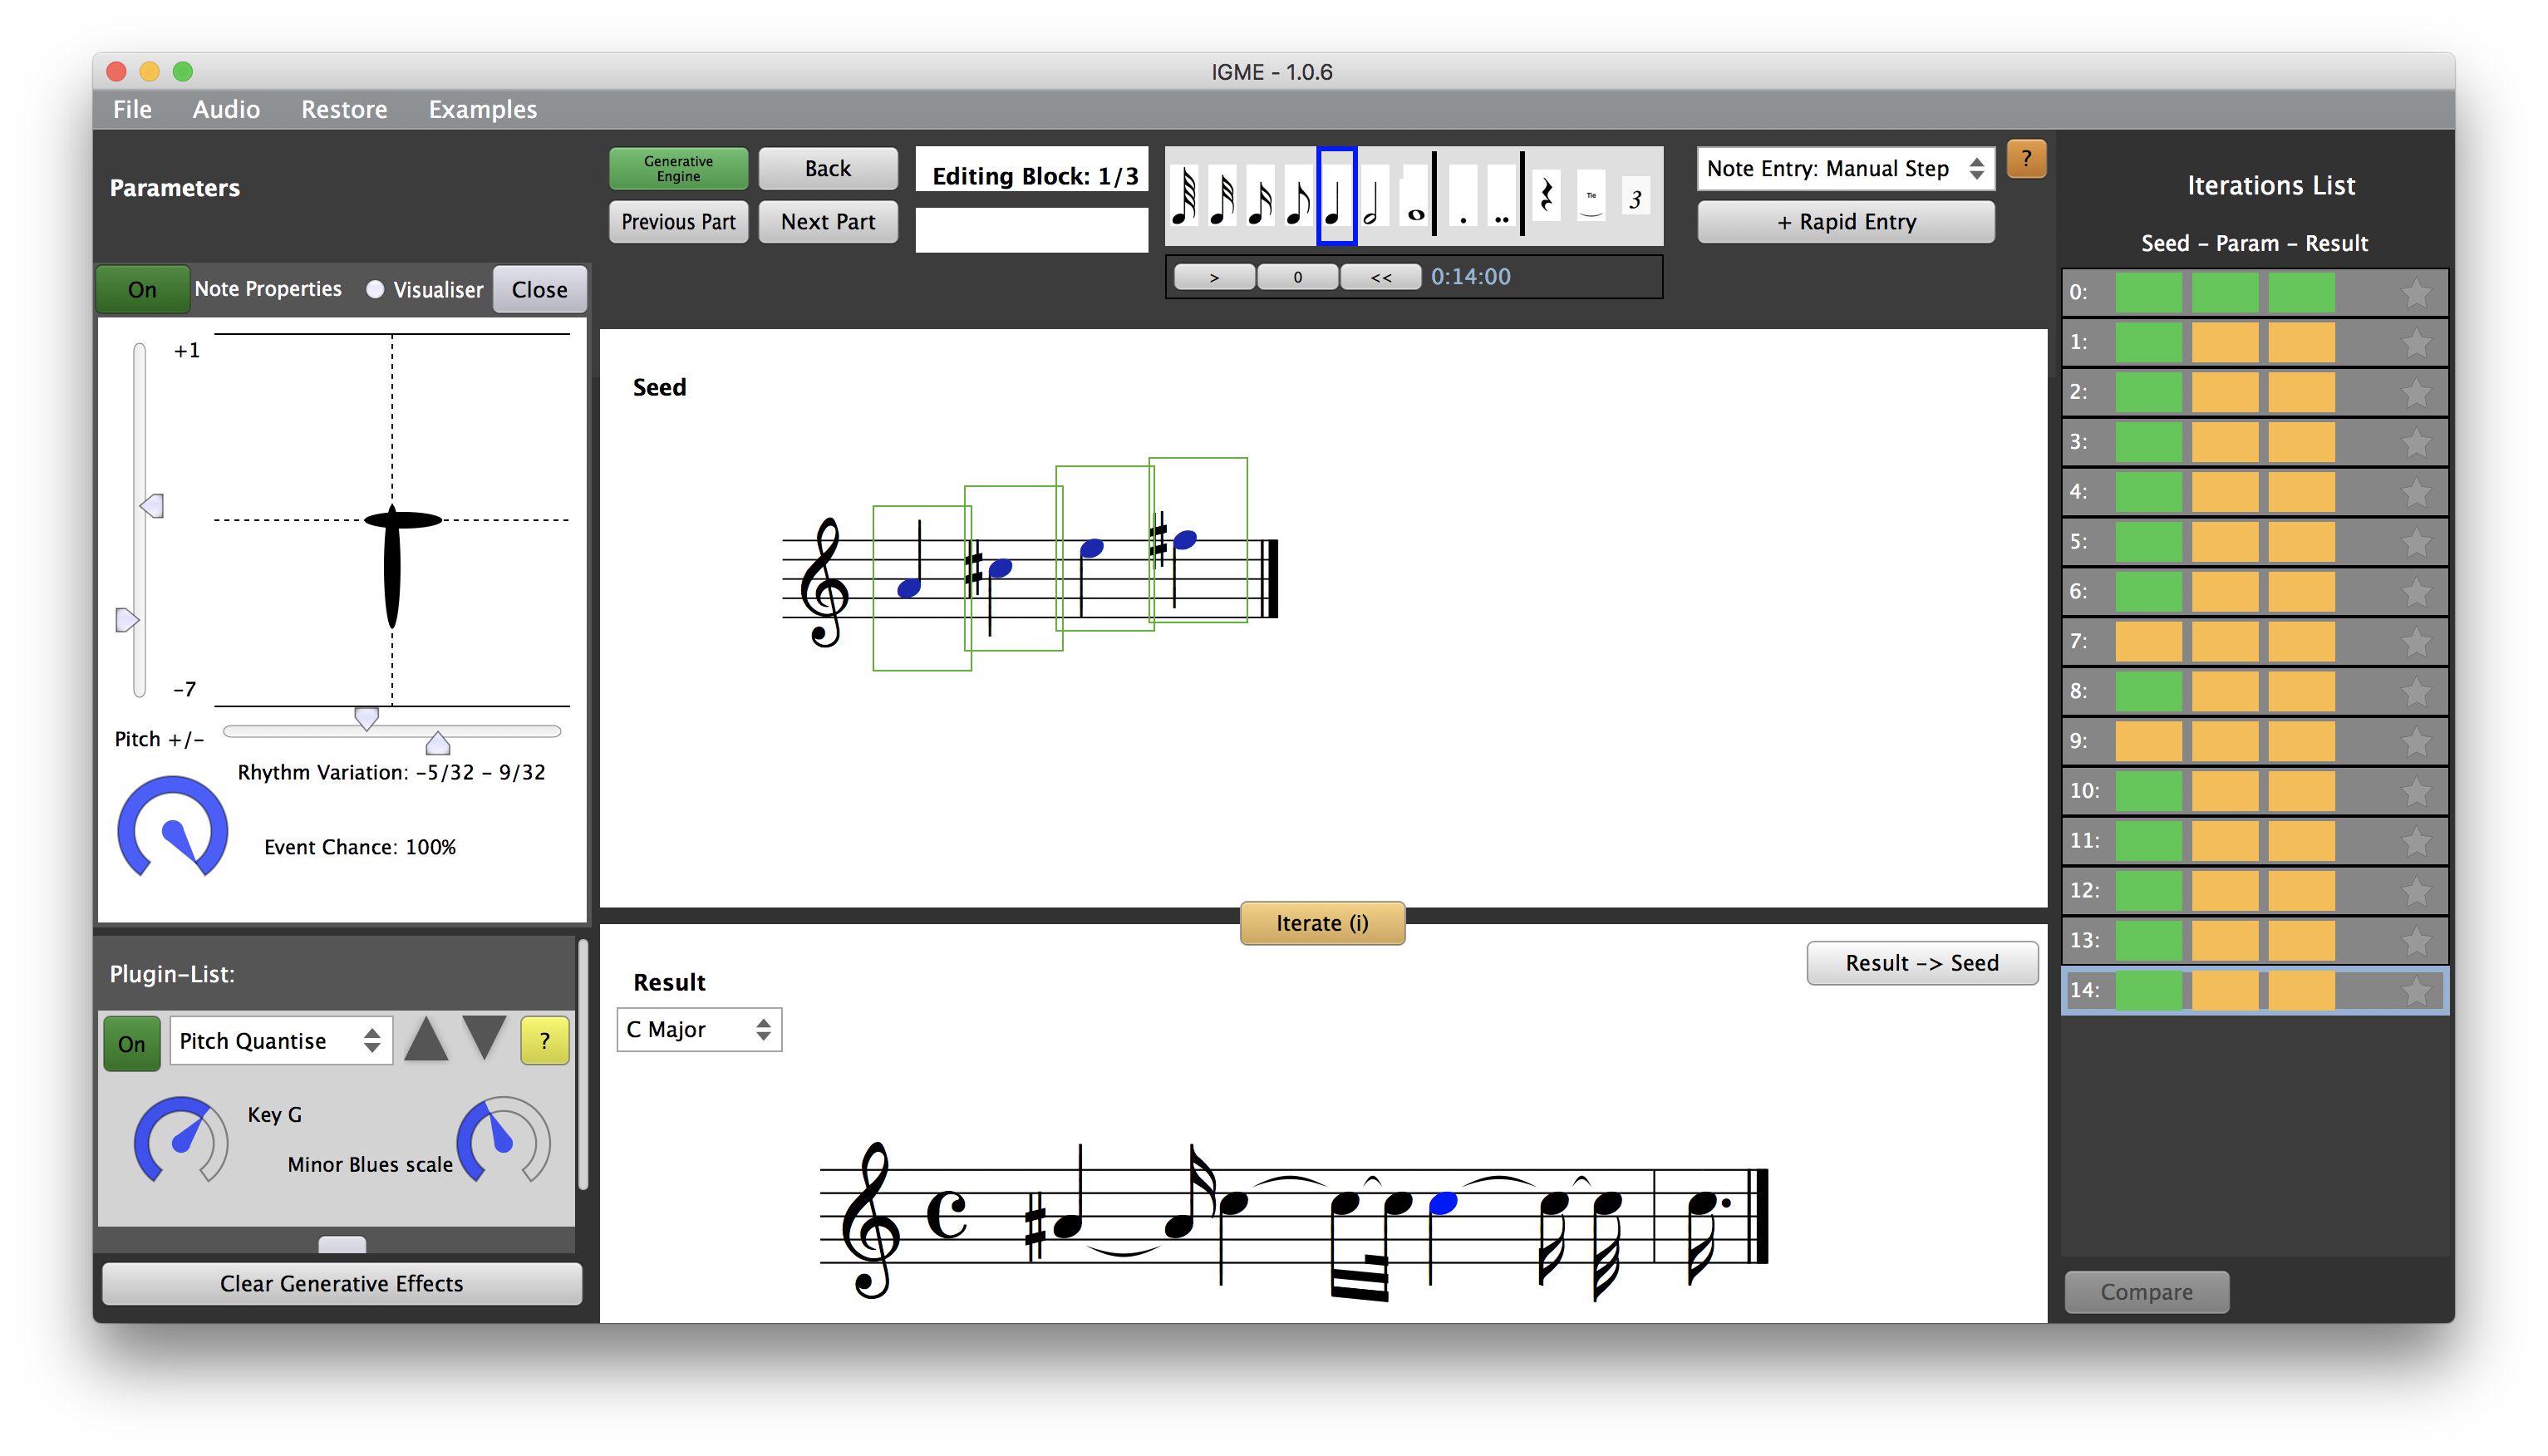
\includegraphics[width=\linewidth]{Images/EditView}
  \caption{Example of an image.}
  \label{fig:igme1}
\end{figure}

\begin{figure}[h]
\begin{center}
  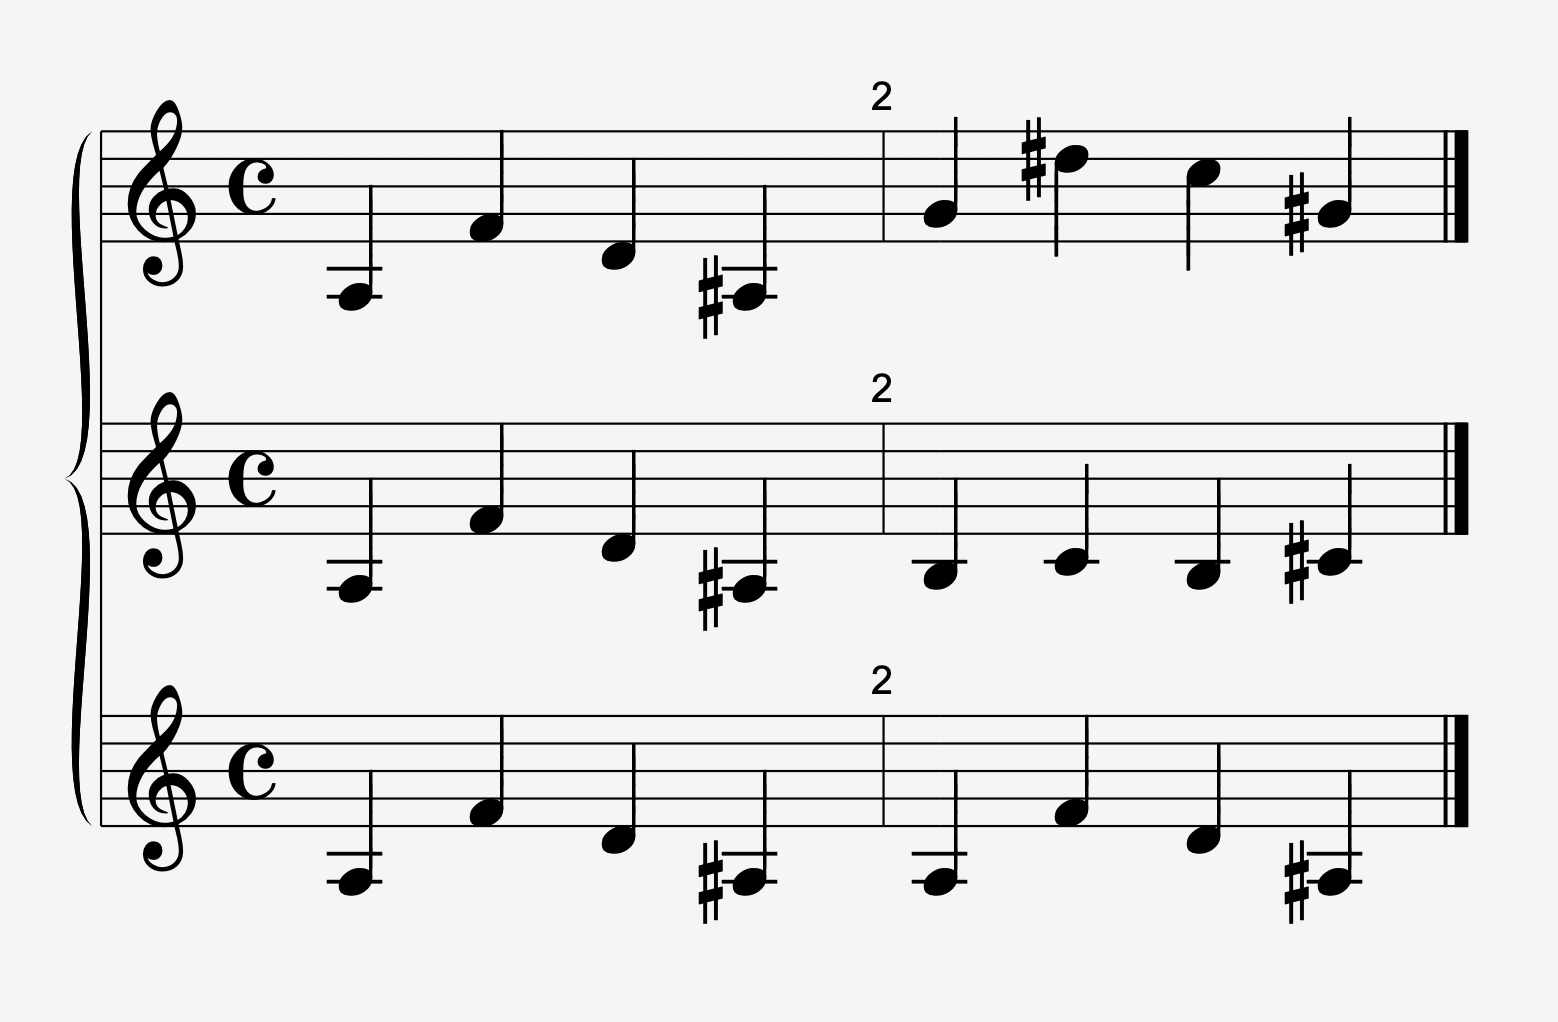
\includegraphics[width=0.6\linewidth]{Chapters/Evaluation/Images/partTypesScore}
  \caption{Another example of an image.}
  \label{fig:igme2}
  \end{center}
\end{figure}


\clearpage

\section{References and Citations}

\LaTeX{} will take care of building your reference list for you. Add your sources to the \textit{``references.bib''} file. Then you can cite using either \verb|\citet{} or \citep{}.| For example.

\begin{itemize}
\item \citet{hunt2020nime} studied interaction in computer-generated music systems - (uses \verb|\citet{}|).
\item IGME was built to study end-user computer-generated music \citep{hunt2020nime} - (uses \verb|\citep{}|).
\end{itemize}

References are automatically formatted as UWE Harvard. 

\subsection{Setup}

You will need to change your bib(la)tex command to use biber: ("biber" \%). This is what my Texmaker settings look like:

\begin{figure}[h]
  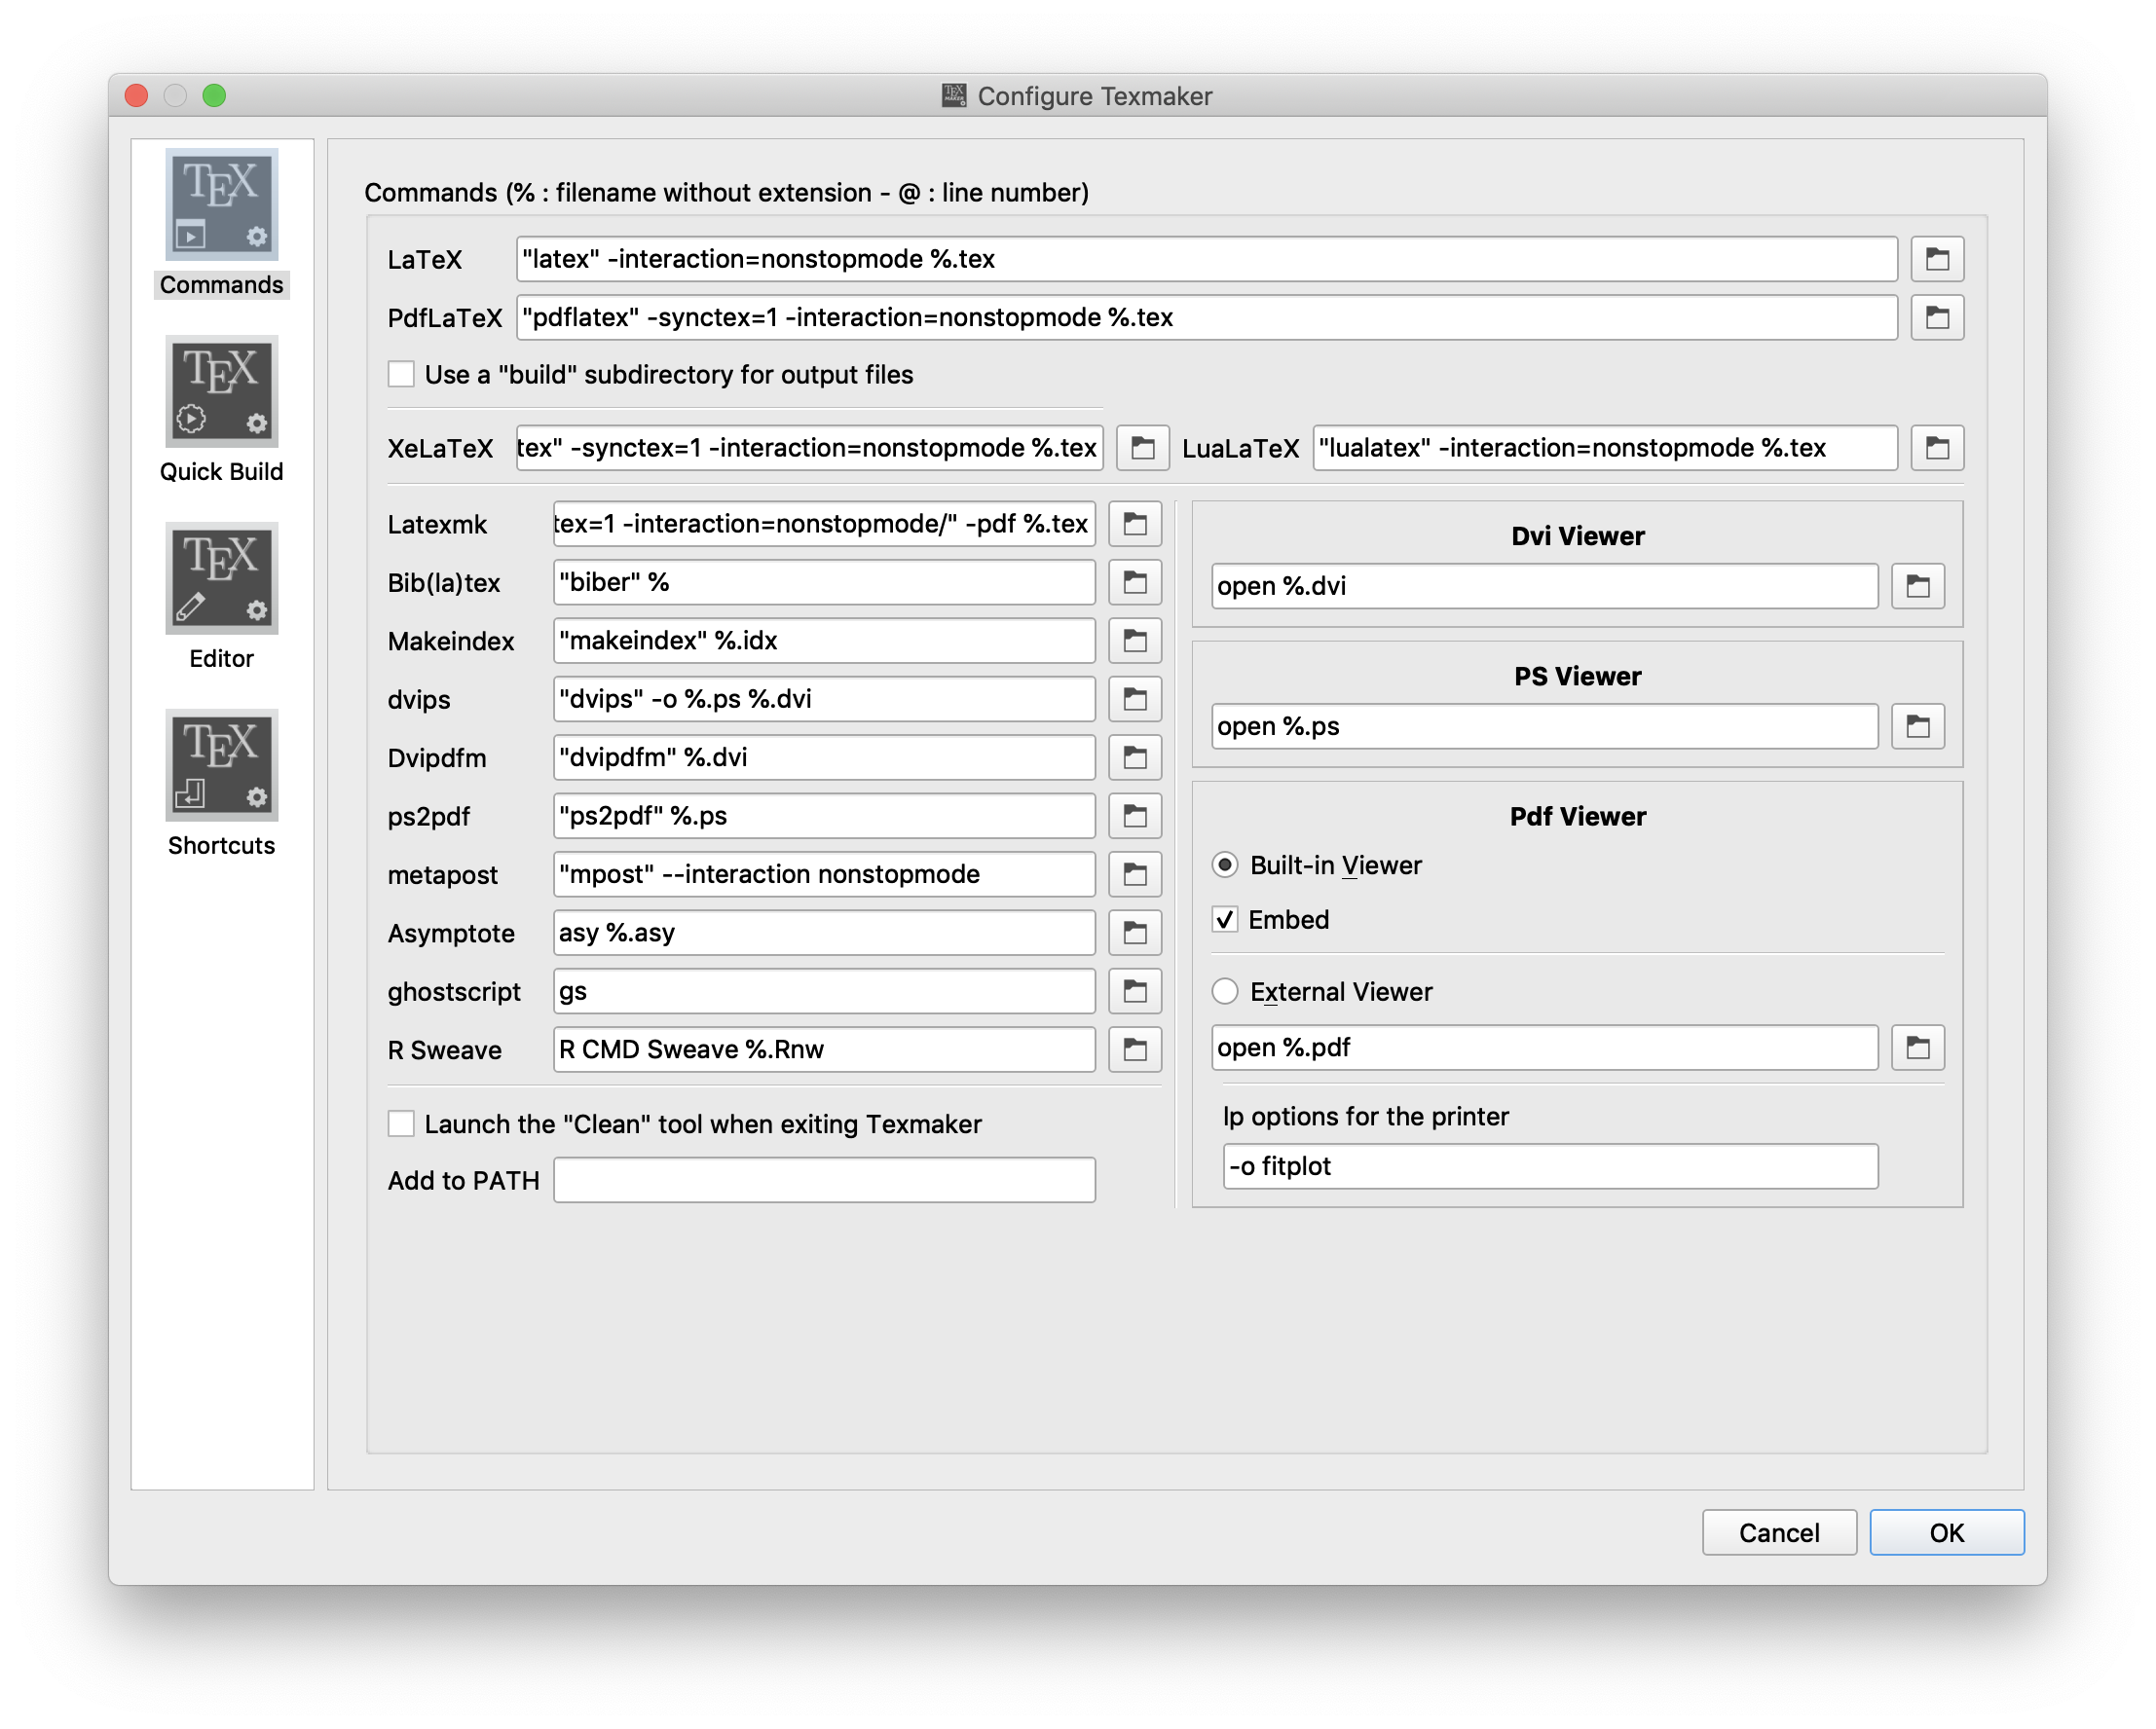
\includegraphics[width=\linewidth]{Images/texmaker}
  \caption{Settings in Texmaker.}
  \label{fig:igme1}
\end{figure}

\section{Building}

To build the thesis use:

\begin{enumerate}
\item XeLaTex
\item bibtex
\item XeLaTex
\item XeLaTex
\end{enumerate}

You can then just use \textit{XeLaTex} to rebuild the thesis, however references, figures numbers, and others wont get updated unless you do the full 4-step process.


 \section{Questions}
 
 Please email sjhunt93@gmail.com for any questions.




%------------------------------------------------------------------------------------
% research
%------------------------------------------------------------------------------------


\part{BACKGROUND} 
%[\textit{The question of whether computers will ever be `creative' in the sense that we speak of creative composing is rather similar to the problem of whether they `think'. Also, we might ask: ``What is meant by the term creative?'' Being `creative' would seem to depend at the very minimum, like `thinking,' on having a computer operate on a self-sustaining basis, and to `learn from experience.' If we postulate, therefore, that creative actions involve, at the very least, a unique perception of relationships between apparently disassociated events in such a way that a new truth is disclosed, then creativity seems to be bound up with the question of ignorance. Moreover, it seems that what we first consider strokes of insight and manifestations of ``creative thought'' are, once they are analyzed and codified and, particularly, codified to the extent that they can be processed by a computer, no longer ``creative processes'' in the usual sense. Seen in this light, the pursuit of knowledge which depends on ``creative thought" is a technique of coding, of finding explicit statements of more and more complex logical relationships. If `creativity' is defined in such terms, then the question of whether machines can do this type of coding is the one which has to be answered. The present computers, even though they may be programmed to process problems in music, for example, cannot be expected to seek out new musical principles. These now must be fed to the machine in explicit detail, and, at best, the uncertainty introduced by freedom of choice, i.e., the use of the random-number processes which we have applied to produce computer music, perhaps gives a computer a very primitive sort of unpredictability, but this can hardly be equated to any sort of creative process.} - \citet{hiller1959experimental}]

\input{Chapters/Research/HCIandCreativity}
\input{Chapters/Research/backgroundGenerativeTechniques}
\input{Chapters/Research/backgroundGenerativeSystems}

%------------------------------------------------------------------------------------
% development
%------------------------------------------------------------------------------------

\part{DEVELOPMENT}
\input{Chapters/Development/designRequirements}
\input{Chapters/Development/IGMESystemDescription}

%------------------------------------------------------------------------------------
% Empical evaluation
%------------------------------------------------------------------------------------

 
\part{EVALUATION}

\input{Chapters/Evaluation/methodologies}
\input{Chapters/Development/IGMECognitive}

\input{Chapters/Evaluation/nime2020paper}
\input{Chapters/Evaluation/LongitudinalStudy}

%------------------------------------------------------------------------------------
% Conclusion
%------------------------------------------------------------------------------------

\part{CONCLUSION}
\chapter{Conclusion}\label{chap:con}


That's a wrap folks!
		
\fi

%------------------------------------------------------------------------------------
% working chapter
%------------------------------------------------------------------------------------

%\input{Chapters/Evaluation/LongitudinalStudy}

\chapter{Introduction}\label{chap:intro}


Welcome to this \LaTeX{} thesis template. This template was originally created by the fabulous Dr Dom Brown, and updated by the amazing but not-quite-Dr Samuel Hunt. This template assumes you already know the basics of \LaTeX{}.


%Some examples of basic \LaTeX{} code are included throughout this chapter.

\section{Organisation}

The files needed for building this thesis are organised into several folders. In the root you will find uwethesis.tex, chapteronly.tex, references.bib and count.sh. 

\begin{itemize}
\item \textit{uwethesis.tex} is the main tex file and links together the individual chapters which are intended to be written as separate .tex files. This is the file that you should run the various compile commands on.
\item \textit{chapteronly.tex} provides a way of working on just a single chapter without needing to recompile everything.
\item \textit{references.bib} is where you should store your sources using a tool such as bibdesk to manage them. 
\item \textit{count.sh} is an optional utility tool for calculating the word count, you will need to update this as you add chapters. You can run this using \textbf{sh count.sh} from a terminal window. 
\end{itemize}



The 4 folders are organised as follows:

%Please use the relevant readme files in each folder, but in summary.

\begin{itemize}
\item Chapters: Contains the main .tex files, one for each chapter. You can also use sub-folders for grouping relevant chapters, i.e. background.
\item Setup: Contains various files for setting up the thesis, also includes .tex files for abstract, acknowledgements, etc.
\item Images: One of two places to store images (optional).
\item Papers: A good place to store your papers that need to be included (as PDFs).
\end{itemize}



\section{Images}

You may want to organise images in one of two ways. Either having one large folder of images, with sub-folders. Or having a image folder alongside each chapter. An example of both is given below:

\begin{figure}[h]
  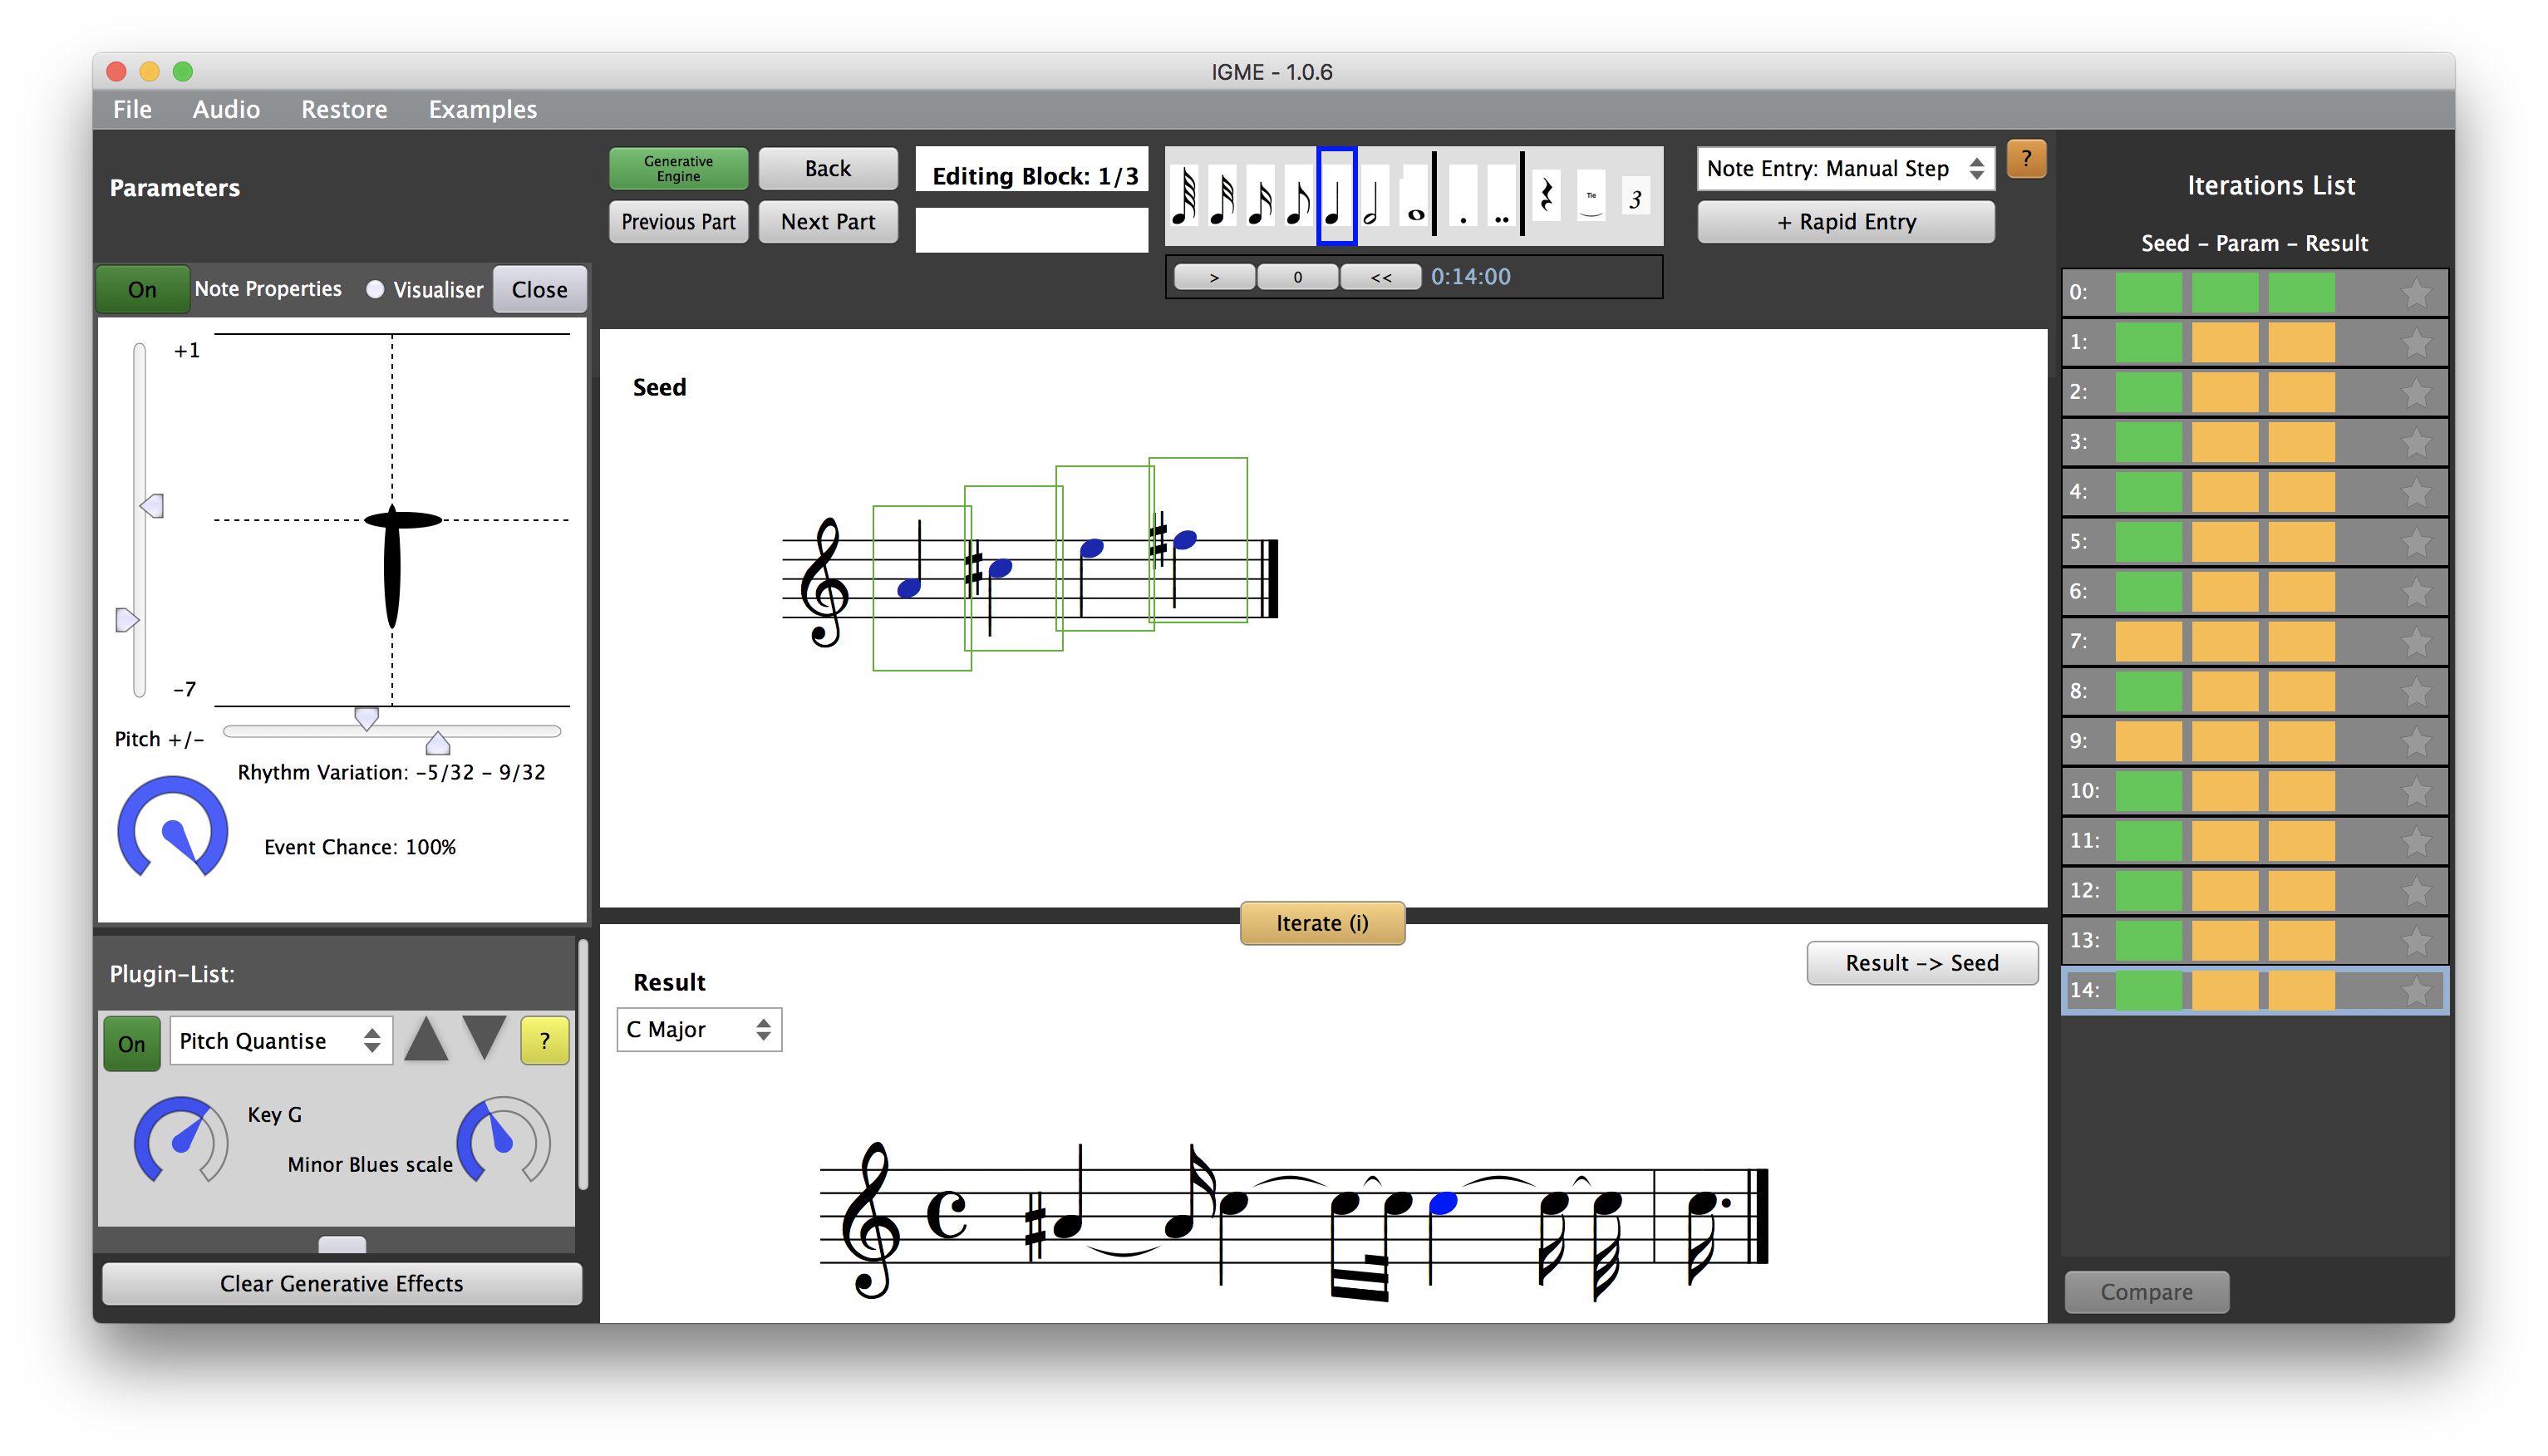
\includegraphics[width=\linewidth]{Images/EditView}
  \caption{Example of an image.}
  \label{fig:igme1}
\end{figure}

\begin{figure}[h]
\begin{center}
  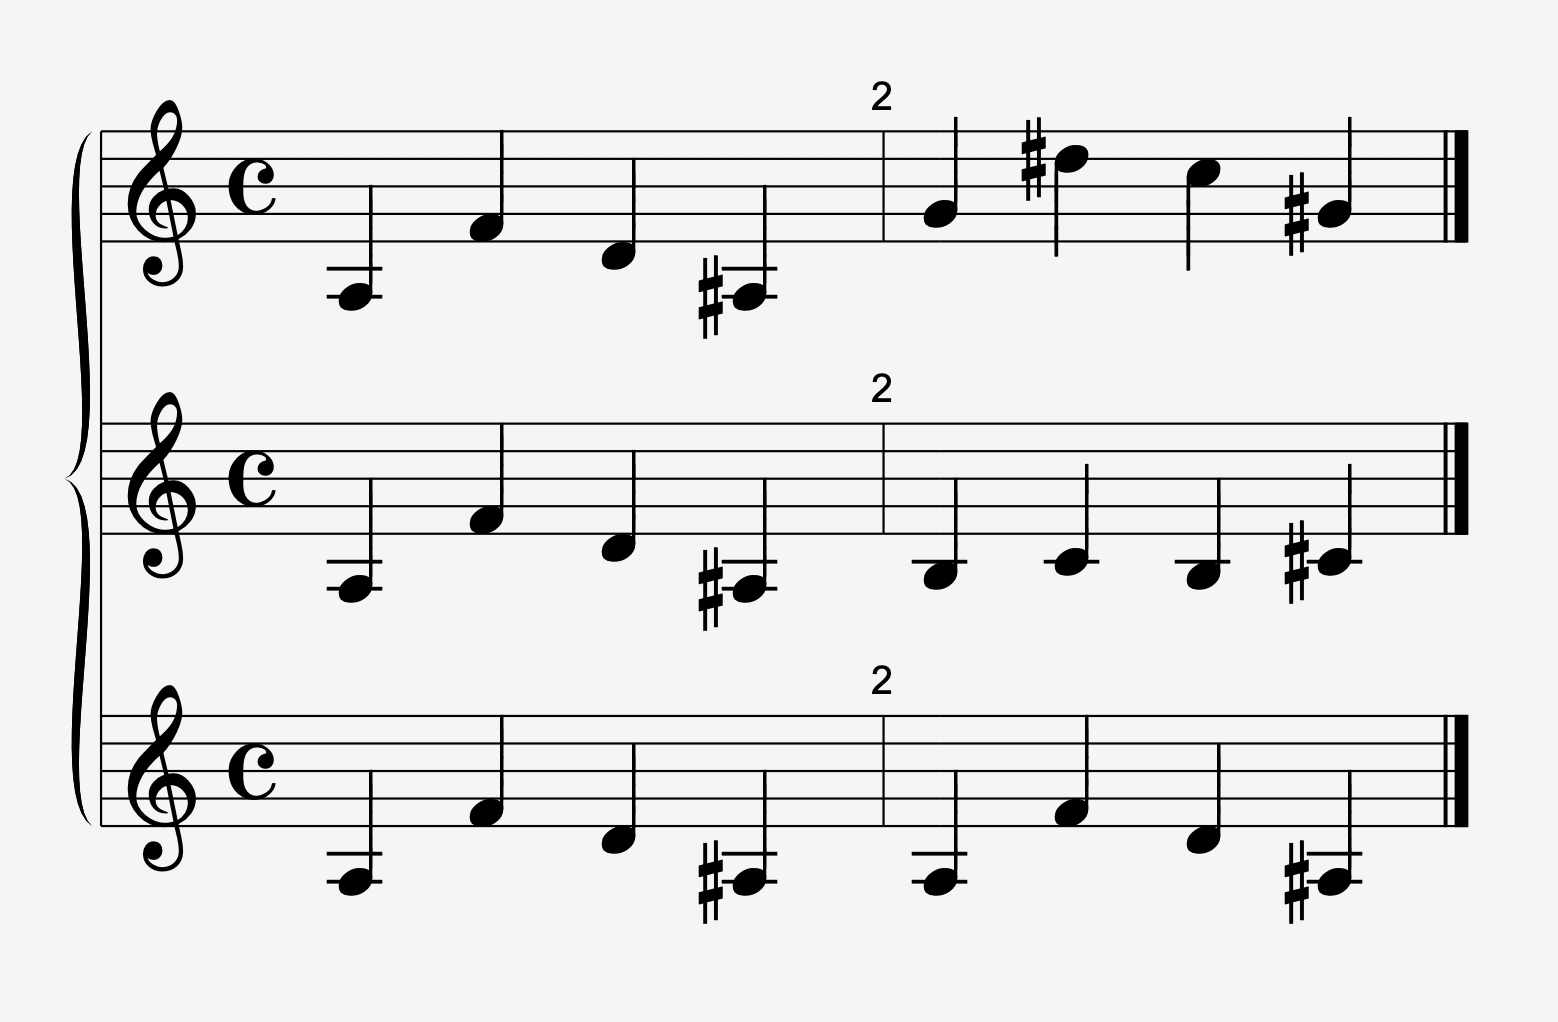
\includegraphics[width=0.6\linewidth]{Chapters/Evaluation/Images/partTypesScore}
  \caption{Another example of an image.}
  \label{fig:igme2}
  \end{center}
\end{figure}


\clearpage

\section{References and Citations}

\LaTeX{} will take care of building your reference list for you. Add your sources to the \textit{``references.bib''} file. Then you can cite using either \verb|\citet{} or \citep{}.| For example.

\begin{itemize}
\item \citet{hunt2020nime} studied interaction in computer-generated music systems - (uses \verb|\citet{}|).
\item IGME was built to study end-user computer-generated music \citep{hunt2020nime} - (uses \verb|\citep{}|).
\end{itemize}

References are automatically formatted as UWE Harvard. 

\subsection{Setup}

You will need to change your bib(la)tex command to use biber: ("biber" \%). This is what my Texmaker settings look like:

\begin{figure}[h]
  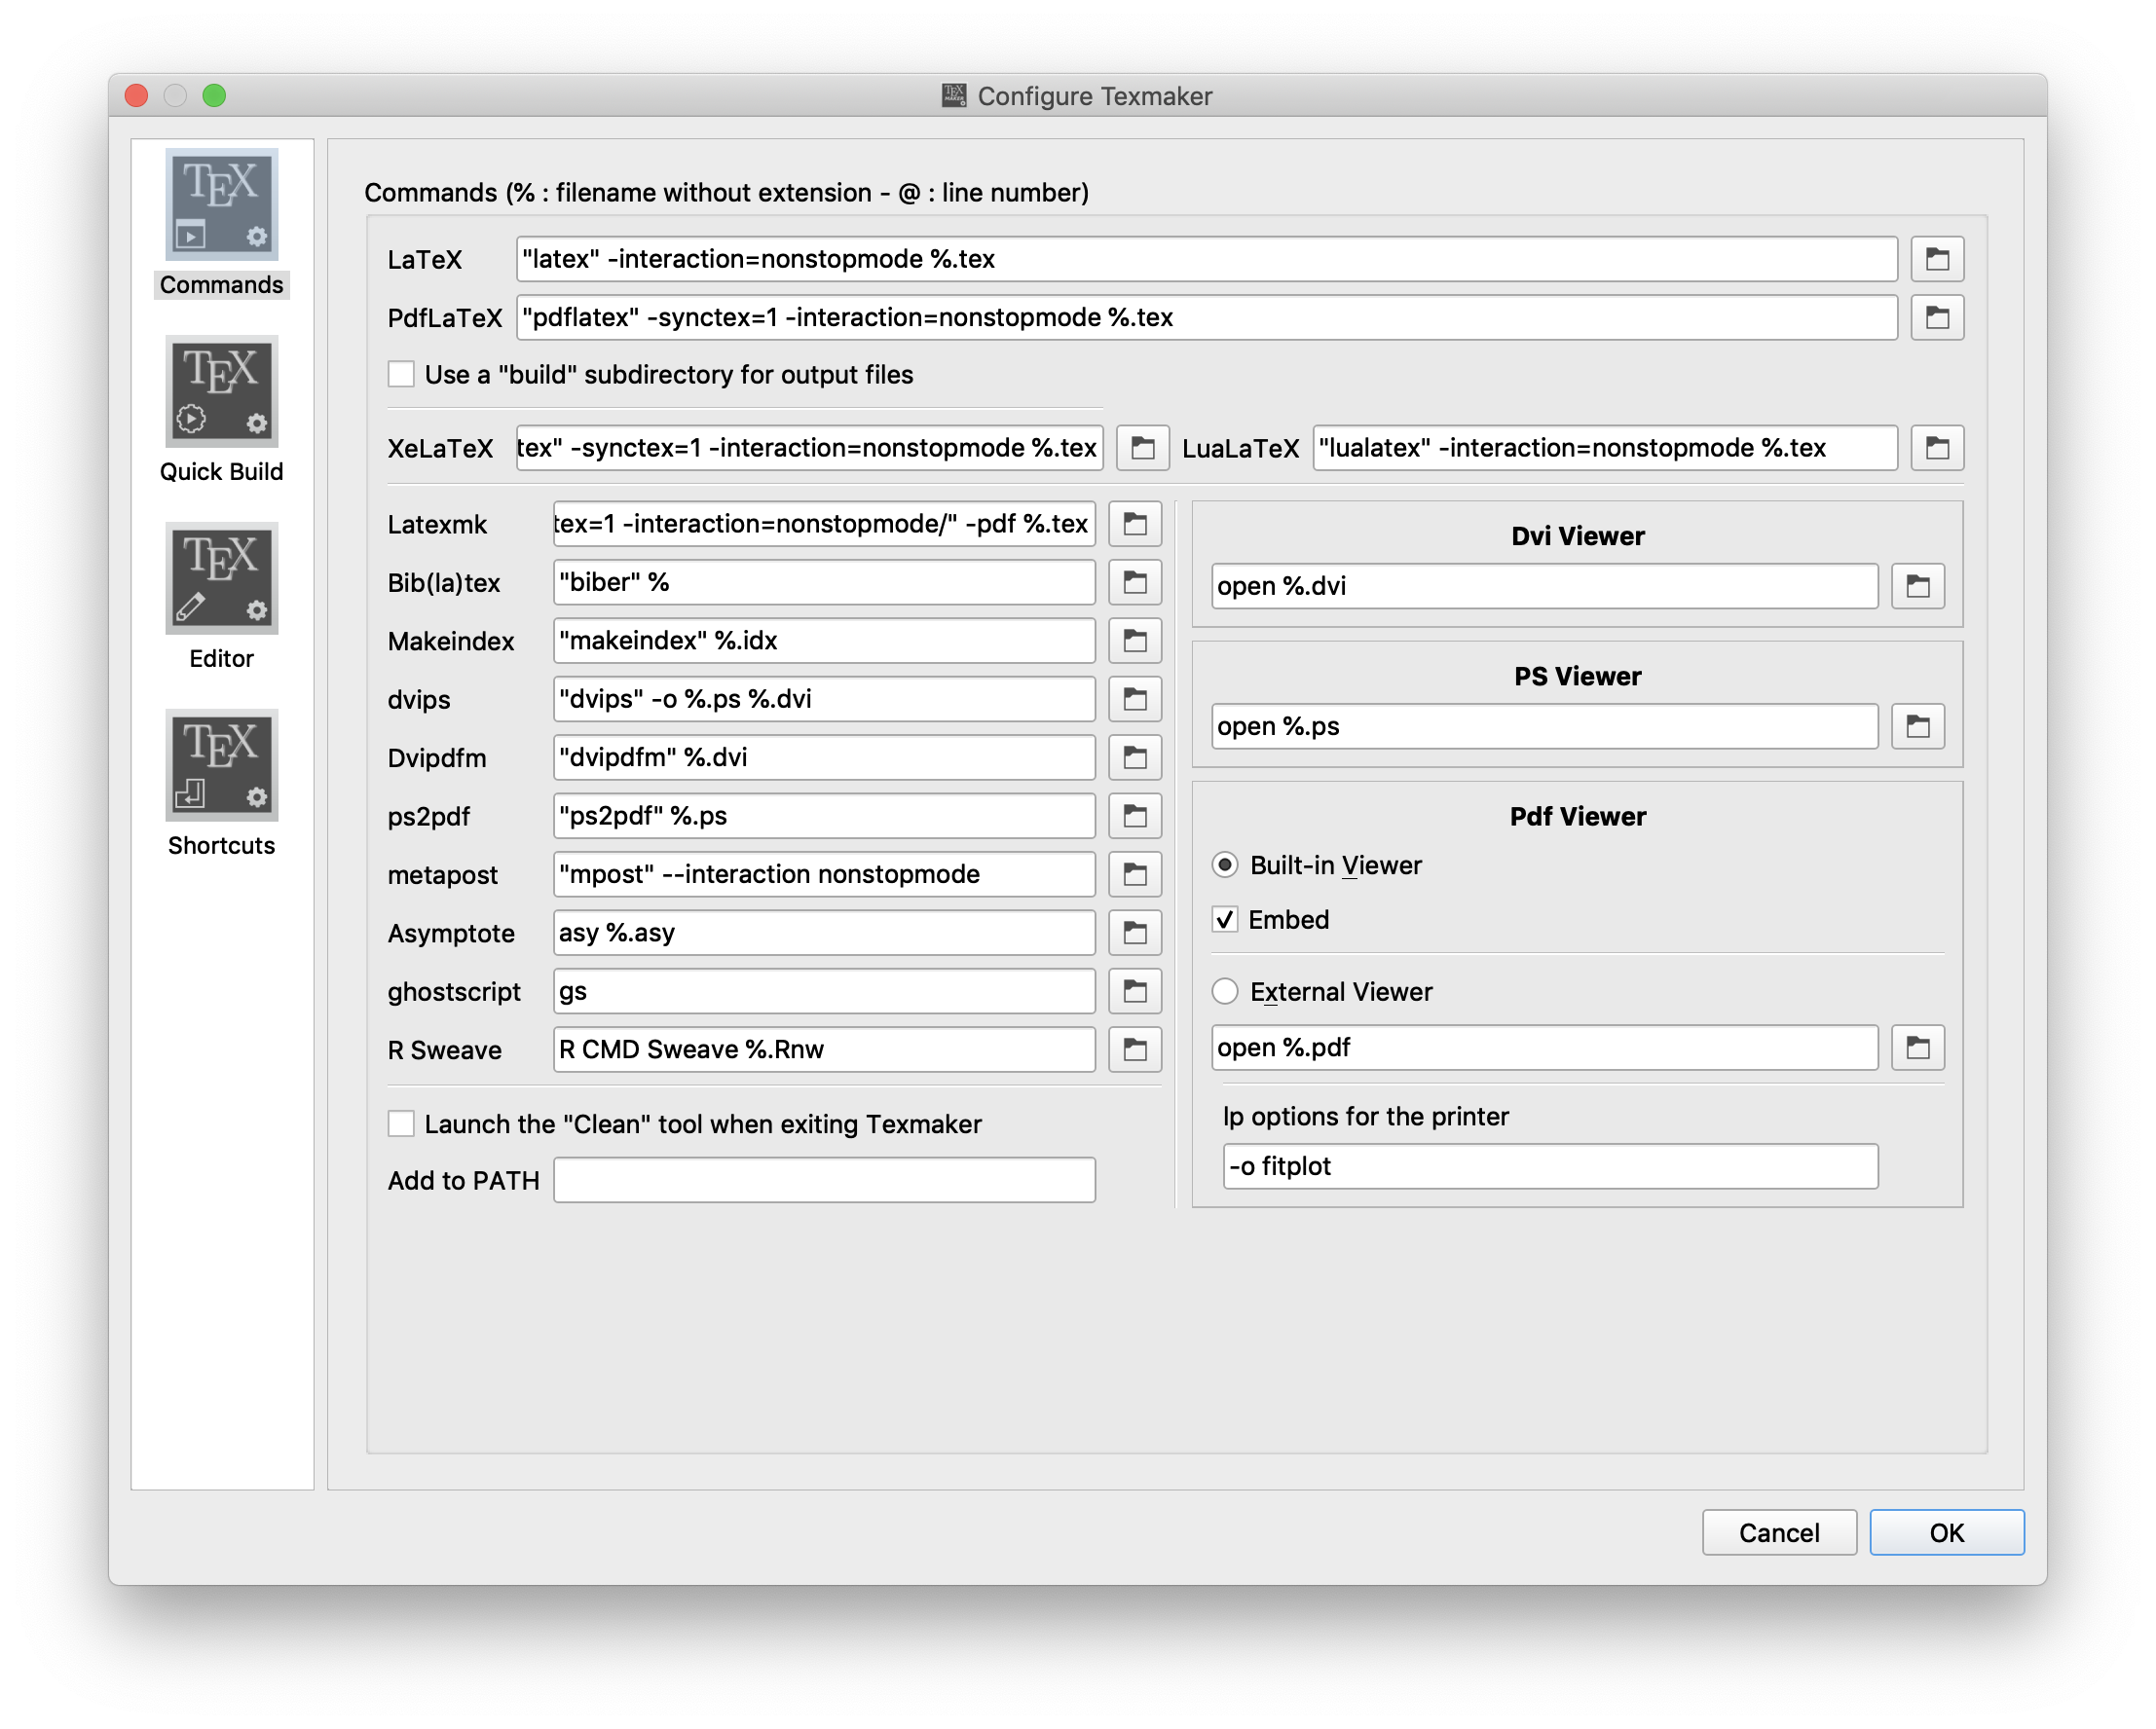
\includegraphics[width=\linewidth]{Images/texmaker}
  \caption{Settings in Texmaker.}
  \label{fig:igme1}
\end{figure}

\section{Building}

To build the thesis use:

\begin{enumerate}
\item XeLaTex
\item bibtex
\item XeLaTex
\item XeLaTex
\end{enumerate}

You can then just use \textit{XeLaTex} to rebuild the thesis, however references, figures numbers, and others wont get updated unless you do the full 4-step process.


 \section{Questions}
 
 Please email sjhunt93@gmail.com for any questions.




%\input{Chapters/appendix/UserSurvey.tex}
%\chapter{Conclusion}\label{chap:con}


That's a wrap folks!

%NIME 2020
% longditudal study
% conclusion



% one could ask waht not only store the seed and generative model. this only works for techniques listed as repoducible (figure \#). However for stochastics systems the output will be different for the same input and generative model, so therefore all three most be considered.


\backmatter
%bibliography
\raggedright
%\onehalfspacing

%\nocite{*}
\printbibliography

\justify


\part{APPENDICES}

\iffalse
%\iftrue

\chapter{Summary}

\subsubsection{A: Music Practitioner Questionnaire}
Discusses the results of a user survey given to music practitioners. Summarised in chapter 5, but discussed at length here. 

\subsubsection{B: Surveys}
Copies of the 3 surveys used in the user studies discussed in chapters 7, 9 and 10.

\subsubsection{C: Existing Music Software Plug-in Summary}
An extension of the work summarised in chapter 4. This section discusses the range of computer-generated plug-ins and processes already in common music software in detail.

\subsubsection{D: IGME System Documentation}
Details all of the computer-generated processes within IGME.

\subsubsection{E: Additional Figures}
Additional figures excluded from the main body.

\subsubsection{F: Additional Publications}
Publications produced as part of doing this PhD that are not discussed in the main body.

\appendix
\addtocontents{toc}{\protect\setcounter{tocdepth}{1}}
\chapter{A: Music Practitioner Questionnaire}

%\chapter{Discussions With Composers}
\label{app:composerSurvey}
\input{Chapters/appendix/UserSurvey.tex}
\section{Survey}
Listed on the next page is the survey given to participants for the work discussed in this chapter.
\includepdf[pages=-,nup=1x2,landscape=true]{Chapters/appendix/SurveyD.pdf}


%\chapter{Appendix Item B: Automating Algorithmic Representations of Musical Structure}
%
%\chapter{Automating Algorithmic Representations of Musical Structure}
%\label{app:igmeAlgo}
%\input{Chapters/Evaluation/algorithmicRepresentations.tex}



\chapter{B: Surveys}
\label{app:survey}
\section{Survey A: Preliminary Evaluation}
\includepdf[pages=-,nup=1x2,landscape=true]{Chapters/appendix/SurveyA.pdf}
\section{Survey B-3: Cognitive Dimensions Evaluation}
\includepdf[pages=-,nup=1x2,landscape=true]{Chapters/appendix/SurveyB3.pdf}
\section{Survey C: Prior Experiences of Music}
\includepdf[pages=-,nup=1x2,landscape=true]{Chapters/appendix/SurveyC.pdf}

\chapter{C: Existing Music Software Plug-in Summary}
\label{app:pluginsum}
\input{Chapters/appendix/AddionalPlugins.tex}

\chapter{D: IGME System Documentation}
\label{app:igme}
\input{Chapters/appendix/IGMEPlugins.tex}

\chapter{E: Additional Figures}
\label{app:extrafig}


\section{Additional Figures}

This section contains additional figures that would otherwise convolute the flow of text in the main body.


%
\chapter{F: Additional Publications}
\label{app:conference}

%The following papers are included as a separate zip folder.
%\iffalse
\section{Tenor 2017: How Can Music Visualisation Techniques Reveal Different Perspectives on Musical Structure}
%\includepdf[pages=-,nup=1x2,landscape=true]{Papers/carbon/TENOR2017.pdf}
\includepdf[pages=-]{Papers/carbon/TENOR2017.pdf}

\section{InMusic 19: Automating Algorithmic Representations of Musical Structure Using IGME: The Interactive Generative Music Environment}
\includepdf[pages=-]{Papers/carbon/inmusic19.pdf}
%\includepdf[pages=-,nup=1x2,landscape=true]{Papers/carbon/inmusic19.pdf}

\section{Audio Mostly 2020: Exploring Polyrhythms, Polymeters, and Polytempi With the Universal Grid Sequencer Framework}
\includepdf[pages=-]{Papers/carbon/AM2020.pdf}
%\includepdf[pages=-,nup=1x2,landscape=true]{Papers/carbon/AM2020.pdf}

\section{CSMC 2020: An Analysis of Repetition in Video Game Music}
%\includepdf[pages=-,nup=1x2,landscape=true]{Papers/carbon/CSMC2020.pdf}
\includepdf[pages=-]{Papers/carbon/CSMC2020.pdf}

%\iftrue
%\section{Tenor 2017: How Can Music Visualisation Techniques Reveal Different Perspectives on Musical Structure}
%\includepdf[pages=-]{Papers/carbon/TENOR2017.pdf}
%
%\section{InMusic 19: Automating Algorithmic Representations of Musical Structure Using IGME: The Interactive Generative Music Environment}
%\includepdf[pages=-]{Papers/carbon/inmusic19.pdf}
%\asfjasf
%\section{Audio Mostly 2020: Exploring Polyrhythms, Polymeters, and Polytempi With the Universal Grid Sequencer Framework}
%\includepdf[pages=-]{Papers/carbon/AM2020.pdf}
%
%\section{CSMC 2020: An Analysis of Repetition in Video Game Music}
%\includepdf[pages=-]{Papers/carbon/CSMC2020.pdf}
%
%
%\fi % finish if for conference papers


\fi



%\section{User Survey}
%\input{Chapters/UserSurvey}

%\end{appendices}



% this is all from doms..
%\appendix
%%\input{Appendices/novice-appendix}
%%\raggedright
%\chapter{Glover Instructions}
%\label{app:gloverinstructions}
%%\includepdf[pages=-]{Appendices/instructions.pdf}
%\input{Appendices/GloverInstructions/instructionsContent.tex}
%
%
%\begin{comment}
%\chapter{Publications}
%
%As per academic regulations, the publications that contain material presented in this dissertation are included in this appendix.
%\\
%\fullcite{nime:2017}
%\\
%\fullcite{moco:2018}
%\\
%\fullcite{digitalcreativity:2018}
%
%\includepdf[pages=-]{Publications/NIME2017_UX.pdf}
%\includepdf[pages=-]{Publications/MOCO-2018-FINAL.pdf}
%\includepdf[pages=2-21]{Publications/DigitalCreativity2018.pdf}
%\end{comment}
%%TC:endignore



\pagebreak

%\includepdf[page=-]{Papers/carbon/TENOR2017.pdf}

%\addtocontents{toc}{\protect\setcounter{tocdepth}{2}}
\end{document}

% audio
% Guns N’ Roses. (1987), [CD], Appetite for destruction, Universal Music.
% Mitsuda, Yasunori. (1995), [video game music], secret of the forest, Square.
